\documentclass[11pt]{scrartcl}

\title{Software Architektur: JBomberman}
\author{Silvan Adrian \\ Fabian Binna \\ Pascal Kistler}
\date{\today{}}

\usepackage[ngerman]{babel}
\usepackage[automark]{scrpage2}
\usepackage{hyperref}
\usepackage{color}
\usepackage[normalem]{ulem}
\usepackage{scrpage2}
\usepackage{graphicx}
\usepackage{tabularx}
\graphicspath{ {./images/} }
\pagestyle{scrheadings}

\clearscrheadfoot
\ihead{
\includegraphics[scale=0.4]{jbomberman}}
\ohead{Projekt: JBomberman}
\ifoot{Software Architektur: JBomberman}
\cfoot{Version: 1.00}
\ofoot{Datum: 01.04.15}
\setheadsepline{0.5pt}
\setfootsepline{0.5pt}

\usepackage{ucs}
\usepackage[utf8]{inputenc}
\usepackage[T1]{fontenc}


\begin{document}
\def\arraystretch{1.5}
\begin{titlepage}
\begin{center}
\vspace{10em}

\includegraphics[scale=2]{jbomberman}
\vspace{10em}
\end{center}
\begin{center}
\huge {Projekt: JBomberman} \\
\huge {Software Architektur}
\end{center}
\begin{center}
\vspace{10em}
\LARGE {Pascal Kistler} \\
\LARGE {Silvan Adrian} \\
\LARGE {Fabian Binna}
\end{center}

\end{titlepage}

\newpage
\section{Änderungshistorie}
\label{sec:Änderungen}

\begin{tabularx}{\linewidth}{l l l l}
\textbf{Datum} & \textbf{Version} & \textbf{Änderung}  & \textbf{Autor} \\
\hline
\textbf{01.04.15} & 1.00 & Erstellung des Dokuments & Gruppe \\
\textbf{05.04.15} & 1.01 & Logische Architektur & Fabian Binna \\
\end{tabularx}

\newpage
\tableofcontents
\newpage

\section{Einführung}
\subsection{Zweck}
Dieses Dokument beschreibt die Software Architektur für das Projekt JBomberman.
\subsection{Gültigkeitsbereich}
Dieses Dokument ist während des ganzen Projekts gültig und wird laufend aktualisiert.
\subsection{Referenzen}
<Liste aller verwendeten und referenzierten Dokumente, Bücher, Links, usw.>
<Referenz auf ein Glossar Dokument, wo alle Abkürzungen und unklaren Begriffe erklärt werden>
<Die Quellen / Referenzen sollten mit dem Word Tool automatisch erstellt werden>
\subsection{Übersicht}
<Übersicht über den restlichen Teil dieses Dokumentes geben und dessen Aufbau erläutern>
 
\section{Systemübersicht}
<Beschreibt die Softwarearchitektur eines Systems und wie sie sich präsentiert (am besten mit einem Bild um eine Übersicht zu ermöglichen) und einzelne Beschreibungen zu den einzelnen Elementen des Systems>
 
\section{Architektonische Ziele \& Einschränkungen}
<Beschreibt die Softwareanforderungen und Objekte, welche einen Einfluss auf die Architektur haben (z.B. Safety, Security, Privacy, Distribution, usw.); Beinhaltet auch eine Beschreibung von Design und Implementationsstrategie, Entwicklungstools, usw.>

\newpage
 
\section{Logische Architektur}
Dieses Package Diagramm zeigt sowol Client, als auch Server. Client und Server sind zwei eigenständige Applikationen, die getrennt ausgeführt werden. Sie verwenden jedoch teilweise die gleichen Packages.

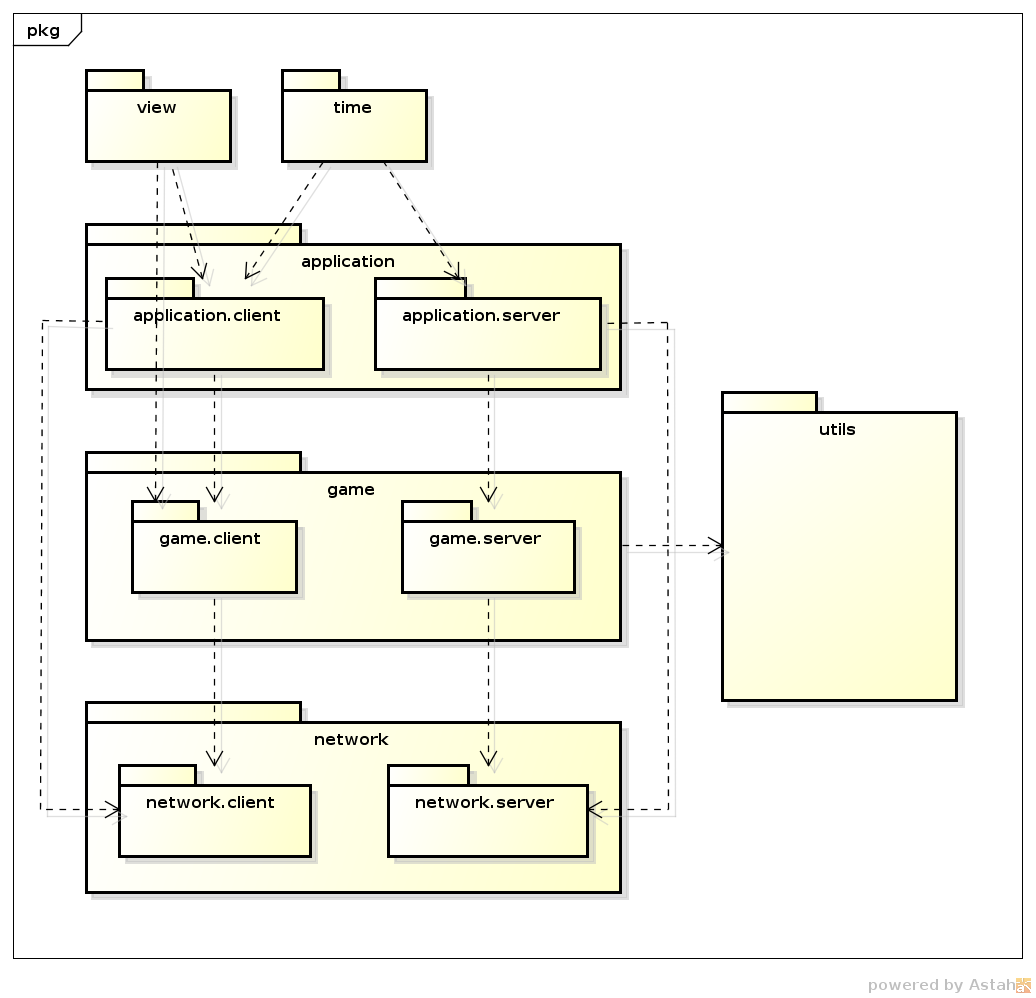
\includegraphics[scale=0.5]{LogischeSicht}

\newpage

\section{Logische Architektur Client}
\subsection{Presentation/view}
Im Package view befinden sich Frames und Canvas, die für die Presentation des Clients notwendig sind.


\subsubsection{Klassenstruktur}
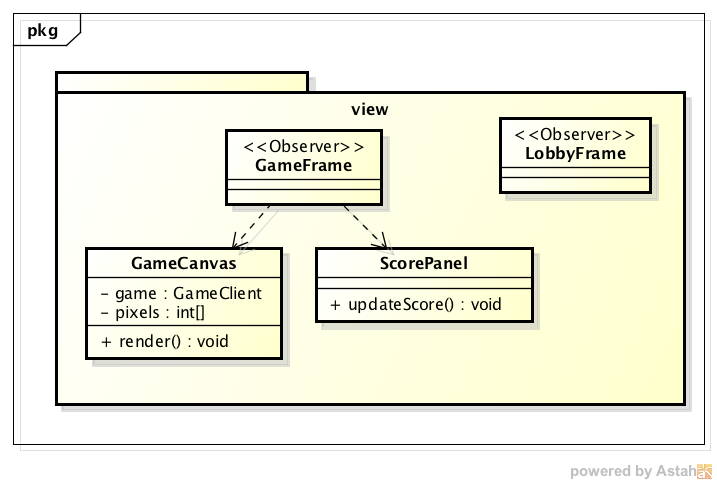
\includegraphics[scale=0.8]{ClassDiagramView}


\textbf{GameFrame}\\
Der GameFrame ist ein Observer und delegiert die Notifies an das zugehörige Panel, die sich dann selber auf den neusten Stand bringen.\\

\textbf{GameCanvas}\\
Der GameCanvas kümmert sich nur um das Rendering, also das Zeichnen der Szene. Dabei delegiert er jedoch nur die pixels[] an alle Sprites, welche sich dann eigenständig zeichnen. Der GameCanvas kümmert sich dann um das performante Buffering.\\\\
\begin{tabularx}{\linewidth}{l p{12cm}}
\textbf{Methode} & \textbf{Beschreibung}\\
\hline
render():void & Kümmert sich um die BufferStrategy und delegiert das zeichnen der Sprites direkt an die Sprites selbst.
\end{tabularx}

\newpage

\subsection{Workflow/application.client}
Im Package application.client befindet sich der workflow des Clients. Er kontrolliert wann der PartyFrame und der GameFrame sichtbar ist.

\subsubsection{Klassenstruktur}
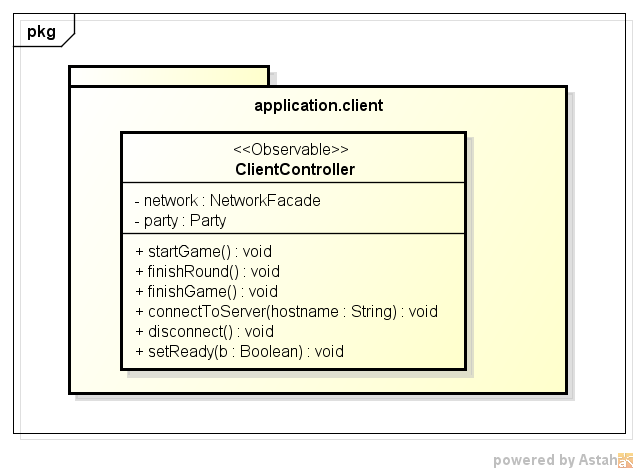
\includegraphics[scale=0.75]{ClassDiagramApplicationClient}

\textbf{ClientController}\\
Der ClientController kontrolliert den Zustand der Client-Applikation. Er notifiziert nur den PartyFrame, nicht aber den GameFrame.\\

\begin{tabularx}{\linewidth}{l p{9cm}}
\textbf{Methode} & \textbf{Beschreibung}\\
\hline
startGame():void & Erstellt eine GameFrame, welches die ClientGame Klasse instanziert und somit das Spiel startet.\\
finishGame():void & Informiert den PartyFrame darüber, dass das Spiel beendet wurde.\\
addPlayer(player: Player) : void & Fügt einen neuen Player in die Party ein.\\
removePlayer(player: Player) : void & Entfernt einen Player aus der Party.\\
connectToServer(hostname: String) : void & Verbindet den Client mit einem RabbitMQ Broker.\\
disconnect() : void & Schliesst die Verbindung mit dem RabbitMQ Broker.\\
setReady(b: Boolean): void & Setzt den Spieler auf bereit.\\

\end{tabularx}

\newpage

\subsection{Domain/game.client}
Im Package game.client werden die Actions vom Server interpretiert und die Sprites auf den neusten Stand gebracht. Die Sprites werden in einer Layer-Logik gespeichet, damit sie korrekt gezeichnet werden können.

\subsubsection{Klassenstruktur}
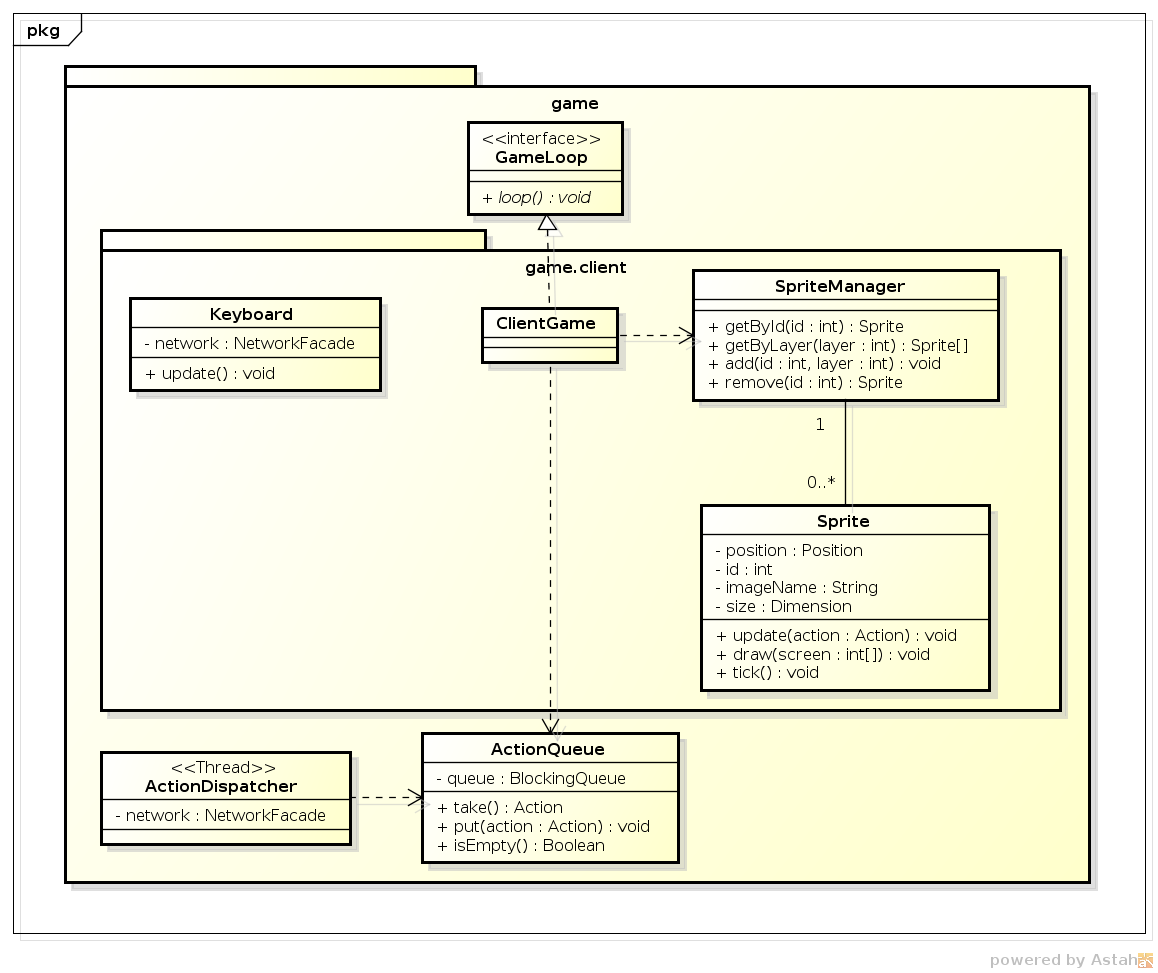
\includegraphics[scale=0.5]{ClassDiagramGameClient}

\textbf{ClientGame}\\
Die Methode loop wird unter "Wichtige interne Abläufe" beschrieben.\\

\textbf{SpriteManager}\\
Der SpriteManager speicher alle Sprites in einer Schichten-Logik. Dies wird benötig, damit die Sprites korrekt gezeichnet werden können. Zudem können die Sprites per id gefunden werden, damit das aktualisieren der Positionen und Zustände einfacher wird. Die Methoden des SpriteManager sind ähnlich wie bei normalen Datenstrukturen und werden deshalb nicht weiter erläutert.

\newpage

\textbf{Sprite}\\
Die Sprite-Klasse beinhaltet alle Informationen die für das Zeichnen der Spielobjekte benötig wird.\\

\begin{tabularx}{\linewidth}{l p{9cm}}
\textbf{Methode} & \textbf{Beschreibung}\\
\hline
update(action : Acton) : void & Interpretiert die Action und führt die nötigen Aktualisierungsschritte durch.\\
draw(screen : int[]) : void & Zeichnet sich selbst auf den screen. Diese Methode wird vom GameCanvas aufgerufen und liefert seinen screen mit auf dem gezeichnet werden kann.\\
tick() : void & Aktualisiert das Sprite. Wird hauptsächlich für Animationen benötigt.\\
\end{tabularx}\\

\textbf{Keyboard}\\
Das Keyboard zeichnet die Tastatureingaben auf und sendet diese direkt über die Methode update an den Server.

\subsubsection{Wichtige interne Abläufe}
//SSD zur GameLoop realisiertung einfügen.


\newpage

\subsection{Network/network.client}

\subsubsection{Klassenstruktur}
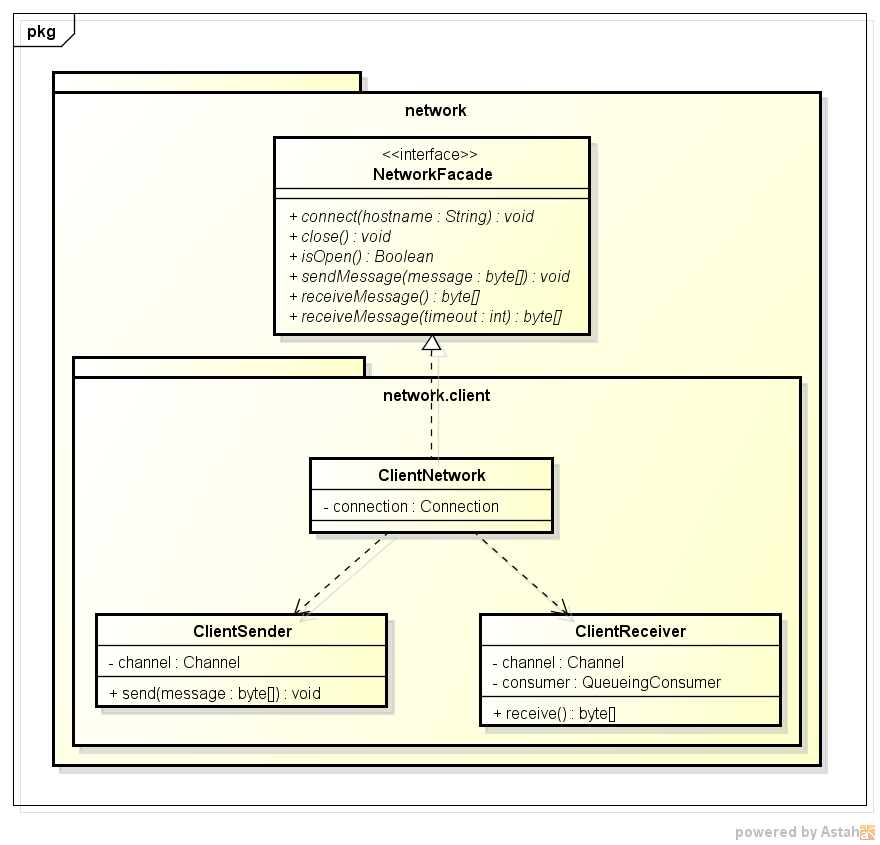
\includegraphics[scale=0.5]{ClassDiagramNetworkClient}




















\subsection{Wichtige Abläufe}
<Beschreibung von wichtigen Abläufen (packageübergreifend)>





 
\section{Prozesse und Threads}
<Wenn mehrere Prozesse oder Threads eingesetzt werden wird hier beschrieben, wie diese ablaufen, miteinander funktionieren, Daten austauschen, sich synchronisieren, usw.>
 
\section{Deployment}
<Beschreibung der einzelnen Komponenten und deren Aufteilung (auf welchen Umgebungen, Servern, usw. laufen die Komponenten)>
 
\section{Datenspeicherung}
<Beschreibung mit Diagramm der Datenspeicherung (Datenmodell, z.B. Datenbank)>
 
\section{Grössen und Leistung}
<Einschränkungen der Applikation bezüglich Speicher, Leistung, etc…. (zum Beispiel: Verwaltung unterstützt maximal 20'000 Einträge)>


\end{document}